% \textbf{Title: Sampling 5}

Consider this spectrum of a sampled signal.

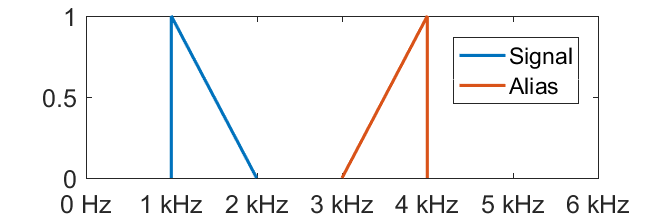
\includegraphics[width=3.45859in,height=1.14589in]{../../Images/SamplingAndAliasingQ5.png}

If we increase the sampling frequency, what could the spectrum of the sampled signal be? \\

a. 

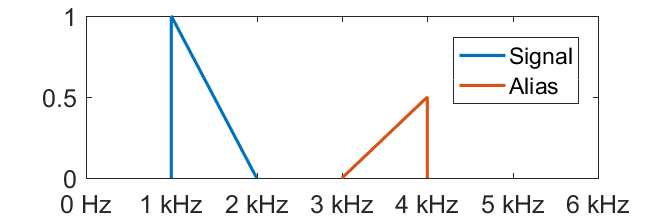
\includegraphics[width=3.49509in,height=1.15798in]{../../Images/SamplingAndAliasingQ5a.png}

%@ Incorrect. This question tests the concept ``Sampling and Aliasing'', which is taught in these courses.

*b.

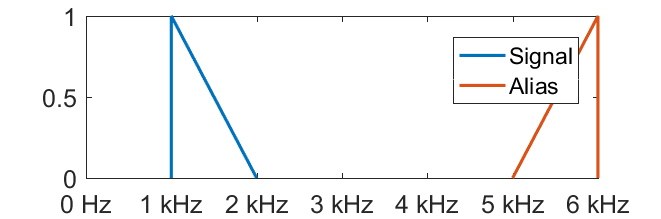
\includegraphics[width=3.50764in,height=1.16214in]{../../Images/SamplingAndAliasingQ5b.png}

%@ Correct! This question tests the concept ``Sampling and Aliasing'', which is taught in these courses.

c. 

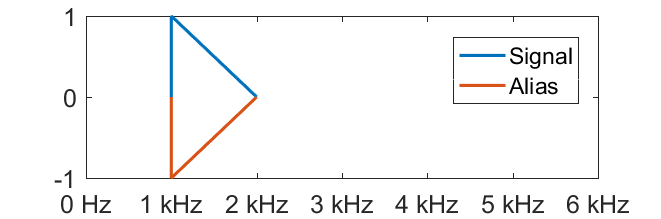
\includegraphics[width=3.64527in,height=1.20774in]{../../Images/SamplingAndAliasingQ5c.png}

%@ Incorrect. This question tests the concept ``Sampling and Aliasing'', which is taught in these courses.

d. 

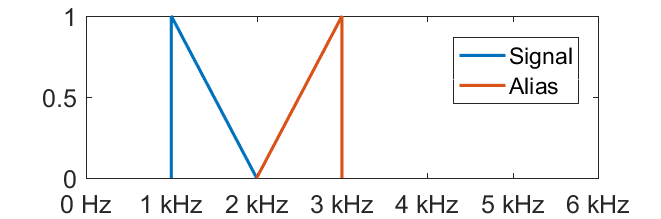
\includegraphics[width=3.60817in,height=1.19544in]{../../Images/SamplingAndAliasingQ5d.png}

%@ Incorrect. This question tests the concept ``Sampling and Aliasing'', which is taught in these courses.

e. I do not know. \\

%@ It's okay. This question tests the concept ``Sampling and Aliasing'', which is taught in these courses.
